\hei{34题}

\qquad \kai{成仿吾是我国无产阶级革命家,马克思主义理论家、教育家,他是由“文化人”成为“革命人”的典型之一。成仿吾究竟是个什么样的人呢?作家丁玲在未跟他谋面之前,曾产生过一系列的“合理想象”:“在文学上,他主张浪漫主义,创造社最早就是这样主张的;他是从日本留学回来的,一定很洋气,很潇洒,因为曾见过一些傲气十足的诗人,趾高气扬,高谈阔论;他在国外学军械制造,或许是庄重严肃之人;他在黄埔军官学校担任教官,一定有一种军人气概;他曾经跟鲁迅进行过革命文学队伍内部的文学论争,写过火气很重的文章,是不是有点张飞李逵式气质呢?”后来,丁玲在陕北见到成仿吾时,第一个感觉就是“我想象的全错 了”。原来成仿吾是一个“土里土气、老实巴交的普通人”,一个尊重别人、热情、虚心、平等待人的人。丁玲十分后悔:“为什么我单单忽略了他是一个经过长征的革命干部、红军战士、一个正派憨厚的共产党员呢?”另据老红军杨定华回忆说,在长征中见到的成仿吾完全是士兵的装扮:破旧的棉军衣,斜挎干粮袋,手持着一枝手杖。杨定华说,成仿吾在红军大学当政治教员。有人说出他的名字,但谁也不知道他是文学家。}

请运用马克思主义认识论基本原理加以分析:

(1)丁玲对成仿吾的“合理想象”为什么“全错了”?

(2)丁玲对成仿吾认识的“转变”过程对我们正确认识事物有何启示?

\clearpage

\hei{35题}

\qquad \kai{多种经济成分并存是当代资本主义和社会主义共有的经济现象。当代资本主义经济中不仅有私有制经济成分,也有国有制经济成分以及其他经济成分;在社会主义经济中不仅有公有制经济成分,也有私有制经济成分以及其他经济成分。但是资本主义和社会主义的基本经济制度的性质是根本不同的。在分析我国社会主义初级阶段生产资料所有制结构问题时,有人以“八宝饭”为例做了形象比喻:八宝饭中的糯米是主要成分,没有糯米不是八宝饭,但糯米本身并不就是八宝饭;八宝饭里还有其他成分,红枣、莲子、核桃、花生、红豆、砂糖等,没有这些成分也不是八宝饭,但这些东西本身也不同于八宝饭。只是把糯米和其他成分组合在一起并以糯米为主才是八宝饭。}

结合材料回答问题:

(1)判断一个社会的基本经济制度性质的根本标准是什么?

(2)我国社会主义初级阶段公有制经济和其他经济成分之间是什么关系?

(3)我国社会主义初级阶段基本经济制度优越性的主要表现是什么?

\clearpage

\hei{36题}

\qquad \kai{减租减息是中国共产党在抗日战争时期解决农民问题的基本政策。减租又称二五减租,即规定地主的地租一律照原租额减收25%,地租的最高额不得超过37.5%。减息的原则是“分半减息”,规定放贷的年利率最高不得超过10%。下表系1942年至1944年对北岳、太行等五个抗日根据地调查的数据。}

\begin{center}\hei{农村各阶层户数及其所占土地的比例(单位:\%)}\end{center}

\begin{center}
	\begin{tabular}{c|c|c|c|c|c|c|c}
	\hline
	\multicolumn{2}{c|}{阶层} & 地主 & 富农 & 中农 & 贫农 & 雇农 & 其他\\
	 \hline
	户数 & 抗战前 & 3.6 & 7.2 & 28.4 & 54.0 & 5.0 & 1.8\\
	\cline{2-8}
	 & 减租后 & 2.4 & 6.7 & 38.0 & 47.0 & 2.5 & 3.4\\
	\hline
	土地 & 抗战前 & 29.5 & 21.0 & 29.5 & 19.0 & 0.8 & 0.2\\
	\cline{2-8}
	 & 抗战前 & 13.5 & 17.5 & 42.5 & 22.5 & 0.6 & 3.4\\
	\hline
	\end{tabular}
\end{center}

结合材料回答问题:

(1)当地土地流向及农村阶级关系发生了什么变化?

(2)简述实行减租减息政策的意义。

(3)解决农村土地问题是新民主主义革命的一项主要任务。结合此表说明减租减息政策的局限性。

\clearpage

\hei{37题}

\hei{材料1}

\qquad \kai{2000年,我国国内生产总值超过了原定比1980年翻两番的目标,这种增长主要是依赖资源的高投入、高消耗来实现的。到2020年实现国内生产总值再翻两番,是我国实现全面建设小康社会的奋斗目标。我国单位GDP消耗的资源能源数量远高于发达国家,也高于印度等发展中国家。按现行汇率计算,2003年我国单位资源的产出水平,只相当于美国的1/10,日本的1/20,德国的1/6。单位产值能耗比世界平均水平高2.4倍,是德国的4.97倍,日本的4.43倍,美国的2.1倍,印度的1.65倍,是世界上单位产值能耗最高的国家之一。而我国人口众多,人均资源比较贫乏,水资源人均占有量仅相当于世界人均的25\%,人均耕地面积不足世界平均水平的50\%,石油人均占有储量为世界平均水平的11\%,大多数矿产资源的人均拥有量不足世界平均水平的50\%。我国环境污染和生态恶化形势十分严峻,1/5的城市空气污染严重,1/3的国土面积受到酸雨影响,全国水土流失面积356万平方公里,沙化土地面积174万平方公里,90%以上的天然草原退化,生物多样性减少。}

\hei{材料2}

\begin{center}
	\begin{tabular}{c|c|c}
	\hline
	\multicolumn{3}{c}{\kai{“十一五”时期资源节约方面的主要指标}}\\
	\hline
	\kai{指标} & \kai{2010年与2005年相比} & \kai{属性(注)}\\
	\hline
	\kai{单位国内生产总值能源消耗} & \kai{降低20\%} & \kai{约束性}\\
	\hline
	\kai{单位工业增加值用水量} & \kai{降低30\%} & \kai{约束性}\\
	\hline
	\kai{农业灌溉用水有效利用系数} & \kai{由0.45增加到0.5} & \kai{约束性}\\
	\hline
	\kai{工业固体废物综合利用率} & \kai{由55.8\%提高到60\%} & \kai{预期性}\\
	\hline
	\end{tabular}
\end{center}

\qquad \kai{注:预期性指标是国家期望的发展目标,主要依靠市场主体的自主行为实现。政府要综合运用各种政策引导社会资源配置,努力争取实现。约束性指示是在预期性基础上进一步明确并强化了政府责任的指标,政府要通过合理配置公共资源和有效运用行政力量,确保实现。}

\begin{center}
\begin{tabular}{c|c|c}
	\hline
	\multicolumn{3}{c}{\kai{"十一五"时期环境保护方面的主要指标}}\\
	\hline
	\kai{指标} & \kai{2010年与2005年相比} & \kai{属性}\\
	\hline
	\kai{耕地保有量} & \kai{减少0.3亿公顷} & \kai{约束性}\\
	\hline
	\kai{主要污染物排放总量} & \kai{减少10\%} & \kai{约束性}\\
	\hline
	\kai{森林覆盖率} & \kai{增加1.8\%} &\kai{约束性}\\
	\hline
\end{tabular}
\end{center}

结合材料回答问题:

(1)中国经济发展面临的资源挑战对经济增长方式转变提出何种要求?

(2)按照科学发展观的要求,我国如何建设资源节约型、环境友好型社会?

\clearpage

\hei{38题}、本题为选做题,请在I、II两道试题中选取其中一道作答,若两题都回答,只按第I道试 题的成绩记入总分。

\vspace{6pt}

\hei{选做题I}

\begin{center}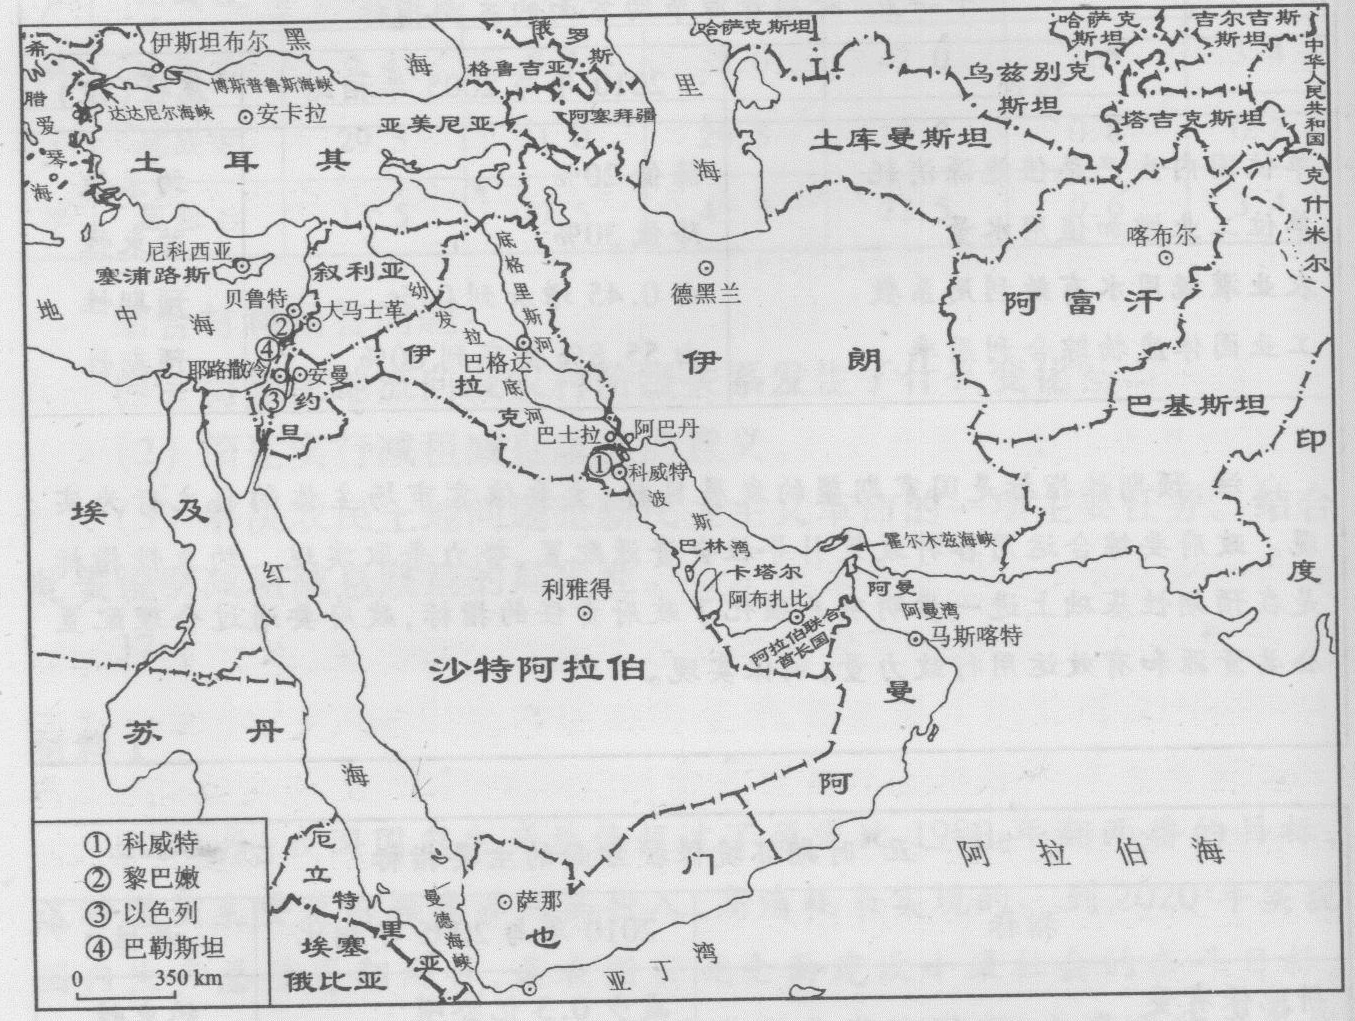
\includegraphics[height=7cm]{pic1.jpg}\end{center}

\begin{center}中东区域示意图\end{center}

\hei{材料1}

\qquad \kai{截止2005年底,世界已探明的石油储量为12000亿桶,其中中东地区为7427亿桶,约占世界总储量的62%。迄今已探明石油储量居世界前列的5个国家沙特阿拉伯、伊朗、伊拉克、科威特和阿拉伯联合酋长国都位于波斯湾地区。中东地区石油产量约占世界总产量的2/5,出口量约占世界总出口量的2/3。}

\hei{材料2}

\qquad \kai{二战后中东局势一直动荡不定,各种地区冲突和局部战争此起彼伏,连绵不断。其中仅阿拉伯国家与以色列之间就进行了5次大规模的战争。而1980年9月发生的两伊战争,则整整打了8年。特别是20世纪90年代初的海湾危机和海湾战争更是牵动了整个世界。时至2003年3月,美、英又对伊拉克发动了一场“先发制人”的战争,迅速占领了伊拉克。2006年7月,黎以之间再次爆发大规模的冲突。至于小规模的武装冲突从未间断过,军事政变、内战和恐怖暗杀等暴力事件也时有发生。可以说,在战后的世界上,没有哪一个地区像中东那样经历如此长期和频繁的战争与冲突。}

结合地图和所给材料分析中东地区持续动荡不安的主要根源。

\vspace{6pt}

\hei{选做题II}

\qquad \kai{坚持包容精神,共建和谐世界。文明多样性是人类社会的基本特征,也是人类文明进步的重要动力。在人类历史上,各种文明都以自己的方式为人类文明进步作出了积极贡献。存在差异,各种文明才能相互借鉴、共同提高;强求一律,只会导致人类文明失去动力、僵化衰落。各种文明有历史长短之分,无高低优劣之别。历史文化、社会制度和发展模式的差异不应成为各国交流的障碍,更不应成为相互对抗的理由。}

\qquad \kai{我们应该尊重各国自主选择社会制度和发展道路的权利,相互借鉴而不是刻意排斥,取长补短而不是定于一尊,推动各国根据本国国情实现振兴和发展;应该加强不同文明的对话和交流,在竞争比较中取长补短,在求同存异中共同发展,努力消除相互的疑虑和隔阂,使人类更加和睦,让世界更加丰富多彩;应该以平等开放的精神,维护文明的多样性,促进国际关系民主化,协力构建各种文明兼容并蓄的和谐世界。}

\begin{flushright}\kai{摘自胡锦涛主席在联合国成立60周年首脑会议上发表的《努力建设持久和平、共同繁荣的和谐世界》讲话}\end{flushright}

结合材料回答问题:

(1)运用辩证法的观点说明为什么不同文明要“在竞争比较中取长补短,在求同存异中共同发展”。

(2)简述中国坚持走和平发展道路对建设持久和平、共同繁荣的和谐世界的意义。
